\documentclass[12pt, a4paper]{report}
\usepackage{graphicx} %LaTeX package to import graphics
\usepackage{enumitem}
\usepackage{geometry}
\usepackage{float}
\usepackage{caption}
\usepackage[list=true,listformat=simple]{subcaption}
\geometry{lmargin=30mm}
\usepackage[export]{adjustbox}
\usepackage{xurl}
\usepackage{titlesec}
\titleformat{\chapter}{\normalfont\huge}{\thechapter}{20pt}{\huge\bf}
\graphicspath{{images/}} %configuring the graphicx package
\title{iasecurity}
\author{Javier Izquierdo Hernández}
\date{\today}
\usepackage[spanish]{babel}
\begin{document}
	\begin{titlepage}
		\centering
		{
\includegraphics[width=0.3\textwidth]{logo}\par}
		\vspace{1cm}
		{\bfseries\LARGE Universidad Rey Juan Carlos \par}
		\vspace{1cm}
		{\scshape\Large E.T.S. Ingeniería de Telecomunicación \par}
		\vspace{3cm}
		{\scshape\Huge DEONTOLOGIA Y NORMATIVA EN ROBOTICA  \par}
		\vspace{3cm}
		{\itshape\Large IA en seguridad bancaria \par}
		\vfill
		{\Large Autor: \par}
		{\Large Javier Izquierdo Hernández \par}
		\vfill
		{\Large \today \par}
	\end{titlepage}

\newpage
\renewcommand{\contentsname}{Contenidos}
\tableofcontents
\listoffigures
\newpage
\chapter{Introducción}
La inteligencia artificial cada vez tiene un uso más habitual en la sociedad, y esto se refleja en la incorporación de esta tecnología en otros ámbitos. En este trabajo vamos a indagar más en profundidad en el uso de IA en la banca por motivos de seguridad y en la prevención de fraudes y estafas. También vamos a tratar el otro lado del espectro con las prácticas que conllevan al fraude y estafas usando la inteligencia artificial.\\

\begin{figure}[h]
	\centering
	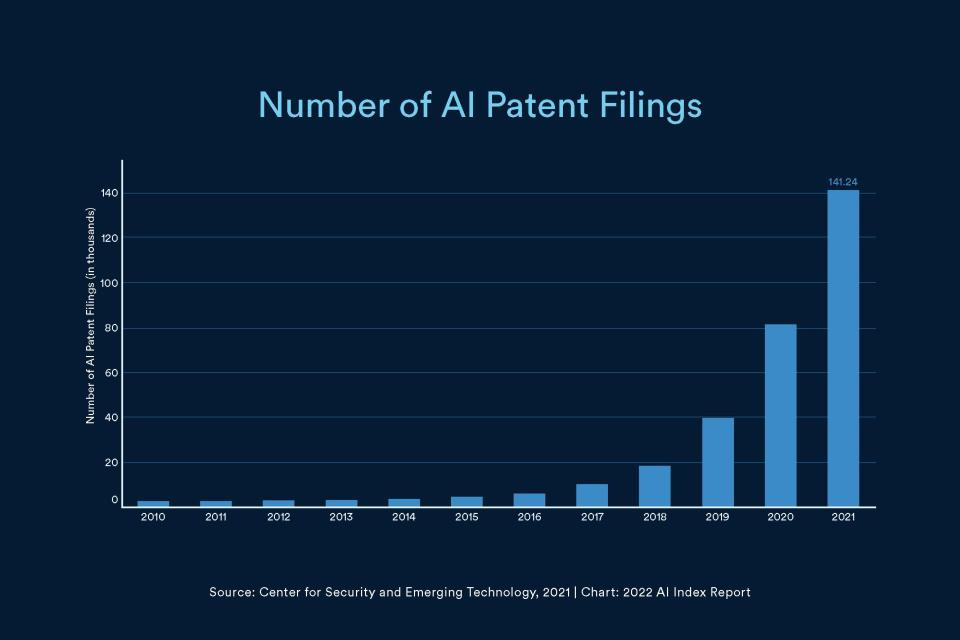
\includegraphics[width=\textwidth]{aipatents}
	\caption{Número de patentes de IA en la última década}
\end{figure}

\chapter{Uso de la IA en la banca}
En la sector bancario se empezó a usar la inteligencia artificial hace unos 5 años aproximadamente, por lo que todavía se encuentra en la fase de desarrollo en muchos bancos.\\
Los usos más principales y donde se hallan los mayores beneficios se pueden dividir en tres partes:
\begin{enumerate}
	\item \textit{Front office}
	\item \textit{Middle office}
	\item \textit{Back office}
\end{enumerate}

La primera parte se encarga del trato con los clientes. Su uso es para intentar solucionar los problemas y necesidades de los clientes de forma autónoma de forma que el cliente quede lo más satisfecho posible, esto se llama \textit{conversational banking}. Véase \ref{chatbot}.
\newline
\begin{figure}[H]
	\centering
	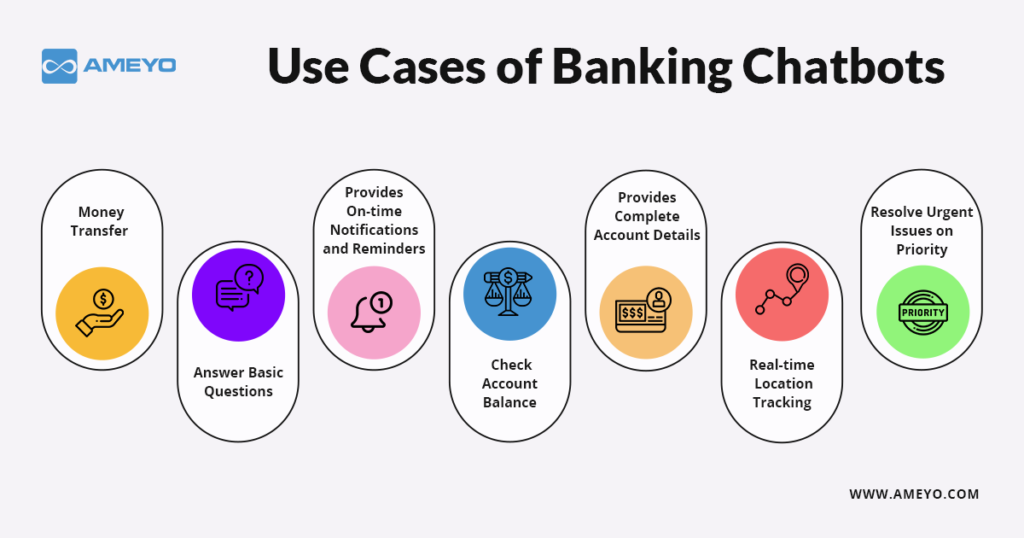
\includegraphics[width=100mm]{usoschatbot}
	\caption{Usos de asistentes en las aplicaciones bancarias}
	\label{chatbot}
\end{figure}

En la siguiente parte ó \textit{middle office} se usa la inteligencia artificial con el fin de reducir el riesgo de fraude y para manejar otros peligros. Esta parte la veremos en más detalle más adelante.
\newline
\newline
Y por último en \textit{back office} se usa para \textit{underwritting}\footnote{Underwriting (cobertura, suscripción de seguro, aseguramiento; dado y aceptado en general después de evaluar riesgos) es el contrato celebrado entre una entidad financiera y una sociedad comercial, por medio del cual la primera se obliga a prefinanciar, en firme o no, títulos valores emitidos por la sociedad, para su posterior colocación. Su existencia se debe a la necesidad de las empresas de obtener recursos financieros y en la actualidad su utilización es cada vez más constante. \\Si bien el contrato de Underwriting se caracteriza por la prefinanciación de los títulos valores, es también parte de la esencia del contrato la prestación de un servicio de asesoramiento previo a la decisión de emitir los títulos. De \cite{wikipedia underwritting}}. A esta parte no entramos más en detalle ya que no se encuentra en el ámbito de este trabajo.
\newline
\newline
Todas estas medidas son tomadas por algunos de los bancos más importantes a nivel mundial, como por ejemplo los mencionados en \cite{url3}:  Capital One, Citi, HSBC, JPMorgan Chase, Personetics, Quantexa y U.S. Bank.

\begin{figure}[H]
	\centering
	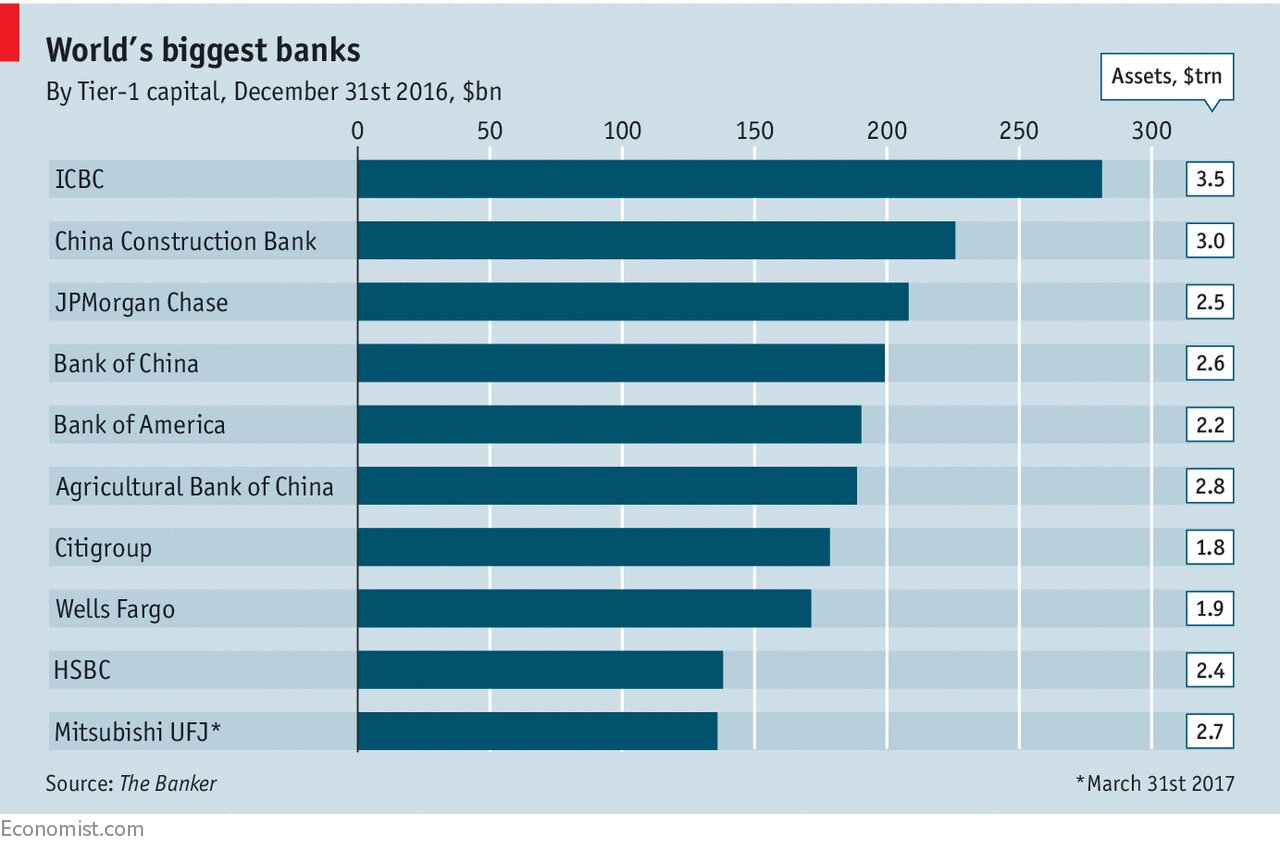
\includegraphics[width=\textwidth]{biggest_banks}
	\caption{Bancos con mayor capital 2016}
	\label{banks}
\end{figure}

\chapter{\textit{Middle office}: control de riesgos}
Los bancos en esta era digital se enfrentan a varias amenazas o riesgos de forma directa o indirecta.

Los riesgos directos son aquellos en los que la propia entidad bancaria sufre perdidas de nivel económico o de reputación. Estos pueden ser:
\begin{enumerate}
	\item Crédito: dar dinero sin saber si este va a ser devuelto. En grandes cantidades esto puede causar a la entidad bancaria a incurrir en una deuda mayor.
	\item Operacionales: errores en las operaciones bancarias pueden causar una brecha en la seguridad o una interrupción del servicio de la entidad.
	\item Mercado: crisis o inestabilidad en ĺa economía global causadas por diferentes causas pueden causar un gran detrimento a la entidad o incluso su disolución. Por ejemplo la crisis del 2008, causo una gran cantidad de perdidas a entidades bancarias y el cierre de varias como Lehman Brothers que causo el estallido de esta.
	\item Liquidez: el banco no puede dar el dinero a sus usuarios de forma inmediata, o a corto plazo.
	\item Ciberseguridad: ataques informáticos con el fin de obtener información sobre el banco y sus usuarios pueden causar una gran pérdida a nivel económico y de reputación, además de un severo problema para sus usuarios que pueden ver sus ahorros desvanecerse.
	\item Reputación: puede ser causado por cualquiera de estos problemas, ya que estos causan descontento a los usuarios. También puede ser causados por una baja satisfacción de los usuarios debido a una mala interacción con ellos por ejemplo en las aplicaciones de banca online. 
	\item Negocio: si un banco no se adecúa a la era actual puede causarle la perdida de usuarios.
	\item Legislativo: si no se adapta a las leyes, esto puede causarle problemas legales que conllevan la perdida de reputación y pueden llegar a causar la disolución de la entidad por incumplimiento de estas leyes.
\end{enumerate}

En estos tipos de riesgos, la inteligencia artificial tiene un factor primordial en multitud de ellos, tales como los: operacionales, de mercado, ciberseguridad, reputación y negocio.
\newline
\newline
Ahora entraremos en detalle en cada uno de ellos para explicar el uso de la IA:

\section{Riesgos Operacionales}
La inteligencia artificial se puede usar con el fin de identificar brechas en el servicio antes de que los humanos puedan percatarse y repararlas antes de que puedan causar un daño mayor.
\section{Riesgos de mercados}
En este ámbito el uso dado a las IA es el de la especulación del estado del mercado global con el fin de poder anticiparse ante las posibles crisis económicas y así sufrir un menor impacto.\\
También es usada para decidir cuales operaciones de capital le dará un mayor beneficio, así como cuales inversiones son más rentables.
\section{Ciberseguridad}
Al incrementar los ataques informáticos de manera exponencial en los últimos años \ref{ciberataques}, una de las maneras más eficientes de protegerse de ellos es usando la inteligencia artificial para la detección y detención de estos. Las IA se pueden usar de diferentes formas como por ejemplo la explicada en el paper \cite{ciber} o en \cite{ciber video}
\begin{figure}[H]
	\centering
	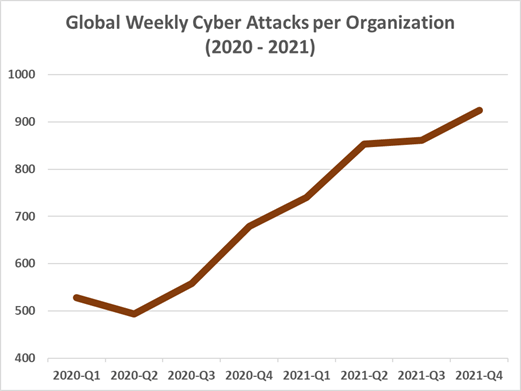
\includegraphics[scale=0.5]{ciberataques}
	\caption{Ciberataques por semana a organizaciones 2020-2021}
	\label{ciberataques}
\end{figure}
\section{Reputación}
Esta parte también incluye la parte de \textit{front office} con las aplicaciones de la IA siendo por ejemplo los asistentes virtuales en las aplicaciones de banca online.
\section{Negocio}
Este parte incluye todas la anteriores. Por ejemplo si un banco no introduce la IA para detener ciberataques, no será capaz de proteger su información por lo que los clientes se irán. Otro sería si no implementan los asistentes virtuales o si no usan la IA para buscar las inversiones más rentables, tendrán un mayor riesgo de perder dinero y reputación.
\chapter{\textit{Middle office}: detección de fraudes}
El fraude es un tipo de riesgo que afecta de forma indirecta a los bancos, pero de forma directa a los usuarios de estos.\\
Las entidades bancarias deciden ayudar a los usuarios a identificar estos fraudes para que ellos se sientan más seguros en depositar su dinero en ellos, en vez de tenerlo guardado en efectivo.
\newline
\newline
Estos fraudes normalmente se basan en un mensaje de teléfono (SMS), en un correo electrónico o en redes sociales en el que se hacen pasar por las entidades bancarias y piden al desconcertado usuario que se dirija a una página web aparentemente de su banco para rellenar unos datos "\textit{necesarios}" para solventar algún tipo de problema en su cuenta. Posteriormente el estafador procede a extraer el dinero de la cuenta del usuario hasta que esta se encuentra vacía, y pasa a la siguiente víctima. Véase \ref{Tipos de estafas}.
\newline
\begin{figure}[H]
	\centering
	\begin{subfigure}[b]{0.35\textwidth}
		\centering
		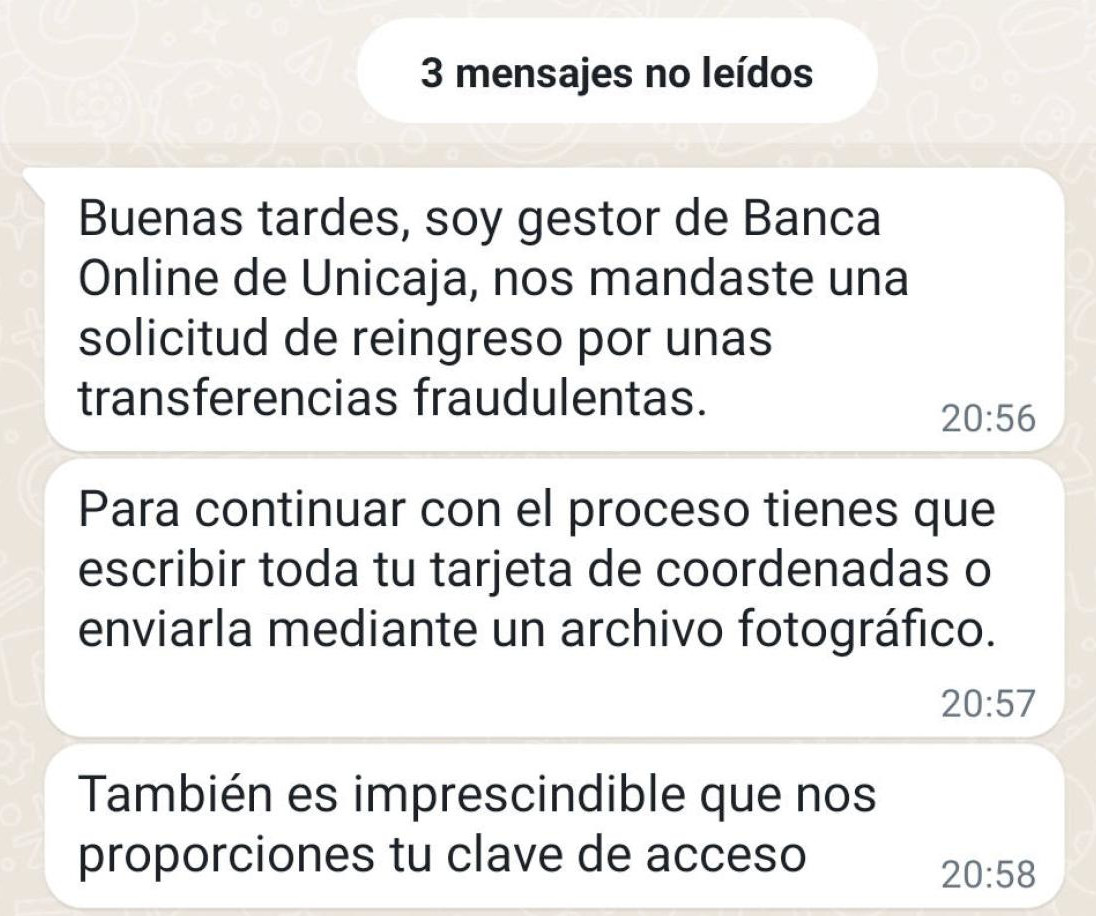
\includegraphics[scale=0.5]{estafa}
		\caption{Estafa Whatsapp}
		\label{Estafa Whatsapp}
	\end{subfigure}
	\hspace{30mm}
	\begin{subfigure}[b]{0.35\textwidth}
		\centering
		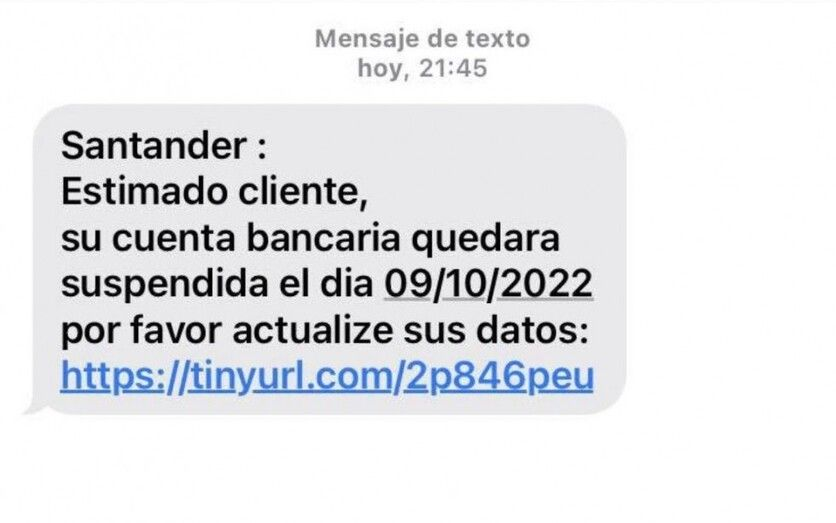
\includegraphics[scale=0.25]{estafa2}
		\caption{Estafa cuenta suspendida SMS}
		\label{Estafa cuenta suspendida SMS}
	\end{subfigure}
	
	\caption{Diferente tipo de estafas y fraudes bancarios}
	\label{Tipos de estafas}
\end{figure}

Viendo este tipo de estafa, los usos que se le podrían dar y se le dan a la IA varían en varios ámbitos:
\begin{itemize}
	\item En los sistemas de mensajería y SMS se usa para diferenciar los mensajes reales de las entidades bancarias de los mensajes fraudulentos.
	\item En las redes sociales al igual que mencionado anteriormente y además para cerrar esas cuentas e identificar a su creador.
	\item En la parte de los bancos una aplicación sería el distinguir las operaciones normales del usuario de las operaciones que haga el estafador, ya sean estas la ip extraña, la velocidad del fin de la transacción desde el inicio de la misma, o el orden de introducción de los campos, etc...
\end{itemize}

El problema que presenta la inteligencia artificial en este caso, es que al igual que se esta usando para intentar impedir estos fraudes, también se esta usando para llevarlos a cabo de manera más convincente y de forma más masiva. Con lo que en este punto se puede considerar como un guerra entre las IA \textit{buenas} que intentan defender al usuario de este tipo de estafas y las IA \textit{malas} que atacan al usuario, decidiéndose esta guerra en cual de las dos IA esta más avanzadas. Para más información sobre esto véase \url{https://www.logicloop.com/fraud-risk/how-fraudsters-can-use-artificial-intelligence-and-chatgpt-to-scam}.
\newline
\newline
También todo esto se podría solucionar con una mayor educación digital a la población para evitar este tipo de fraudes, al menos por ahora.
\chapter{Conclusión}
Ahora mismo estamos en un \textit{boom} del desarrollo de la IA y lo que ahora nos parece imposible dentro de unos meses o años la inteligencia artificial será capaz de ello.\\
\newline
\newline
Por esto mismo el desarrollo de la IA en el campo de las finanzas y del los bancos tendrá que ser consecuente con el desarrollo global, ya que cuanto más avance la inteligencia artificial, más difícil será de protegerse de los ataques informáticos que usen a la misma, lo que obligará a todas estas empresas a protegerse usando la IA con ese fin.
\newline
\newline
A su vez con el intento de desarrollo de AGI (\textit{artificial general intelligence}), no se sabe donde estará el techo de los asistentes virtuales que se usan actualmente en las aplicaciones bancarias y mucho más que nos deparan los próximos años, si estas IAs no son prohibidas por los gobiernos del globo, véase \cite{ban}.
\begin{figure}[H]
	\centering
	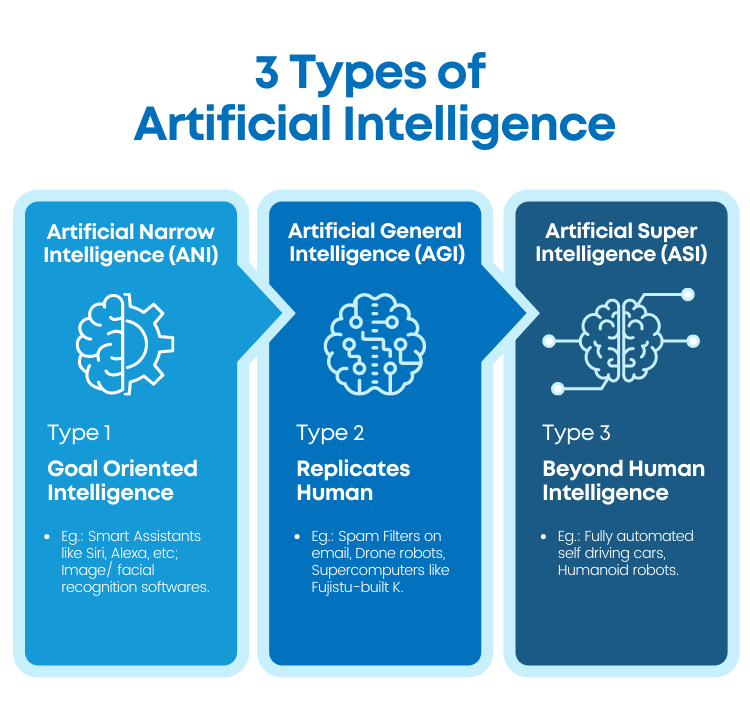
\includegraphics[scale=0.37]{agi}
	\caption{Tipos de IA}
	\label{Tipos de IA}
\end{figure}
\begin{thebibliography}{9}
	\bibitem{url1}
	\url{https://www.insiderintelligence.com/insights/ai-in-finance/}
	\bibitem{url2}
	\url{https://hai.stanford.edu/news/state-ai-9-charts}
	\bibitem{url3}
	\url{https://www.businessinsider.com/ai-in-banking-report}
	\bibitem{url4}
	\url{https://www.inscribe.ai/financial-risk-management/how-banks-manage-risks#:~:text=Banks%20develop%20risk%20management%20programs,prevent%20them%20from%20re-emerging.}
	\bibitem{wikipedia underwritting}
	\url{https://es.wikipedia.org/wiki/Underwriting#:~:text=Underwriting%20(cobertura%2C%20suscripción%20de%20seguro,por%20la%20sociedad%2C%20para%20su}
	\bibitem{ciber}
	\url{https://www.datarobot.com/resources/ai-in-cybersecurity/}
	\bibitem{ciber video}
	\url{https://www.ibm.com/security/artificial-intelligence}
	\bibitem{fraud}
	\url{https://www.logicloop.com/fraud-risk/how-fraudsters-can-use-artificial-intelligence-and-chatgpt-to-scam}
	\bibitem{ban}
	\url{https://www.reuters.com/technology/germany-principle-could-block-chat-gpt-if-needed-data-protection-chief-2023-04-03/}
	
\end{thebibliography}
\end{document}
